\documentclass[../report.tex]{subfiles}


\definecolor{dkgreen}{rgb}{0,0.6,0}
\definecolor{gray}{rgb}{0.5,0.5,0.5}
\definecolor{mauve}{rgb}{0.58,0,0.82}

\lstset{frame=tb,
  language=Sql,
  aboveskip=3mm,
  belowskip=3mm,
  showstringspaces=false,
  columns=flexible,
  basicstyle={\small\ttfamily},
  numbers=none,
  numberstyle=\tiny\color{gray},
  keywordstyle=\color{blue},
  commentstyle=\color{dkgreen},
  stringstyle=\color{mauve},
  breaklines=true,
  breakatwhitespace=true
  tabsize=3
}

\begin{document}

\graphicspath{{img/}{../img/}}

When designing the data model there were several considerations to make. The design goals for the data model were as follows:
\begin{itemize}
\item Make a generic and flexible data model that can easily adapt to accommodate new functionality. 
\item Make the model as extendible as possible. Meaning new properties can be added to e.g. a \textit{Media item} without having to change the data model. This facilitates more iterative development.
\item The data model should be in the highest normal form possible to avoid redundancy in regards to data space and corruption
\end{itemize} 

The first and second design goals stem from the non-functional requirements NFR-07 and NFR-08. These requirements specify that addition of new functionality and new types of media must be supported. In order to meet those requirements a flexible and extendible data model is required.
The third design goal stems from the non-functional requirement NFR-04 which states that corrupt data must not reach the \textit{End User}s. A big part of meeting that requirement is to minimize the chance of data getting corrupted in the first place.

%Firstly it was important to design a data model which was generic enough to accommodate the demands of the SMU team. Secondly it was important to design a data model which was in as high a normal form as possible in order to reduce redundant data and the possibility of creating corrupt data. Lastly we wanted to make the datamodel as extendible to new features as possible.  


%(WHY DID WE MAKE THE UPLOADER/OWNER OF A MEDIA ITEM A RELATION?!? NOW IT IS POSSIBLE FOR A MEDIA ITEM TO HAVE MORE THAN ONE UPLOADER/OWNER)


\textit{The System} revolves around two major entities, namely the \textit{User} and \textit{Media item} (modelled as entity). Additionally it became clear that an entity representing a \textit{Client} was needed in order for the \textit{ShareIt Back End} to be able to differentiate which \textit{Media Item}s belonged to which \textit{Client}. \\


\begin{figure}[H]
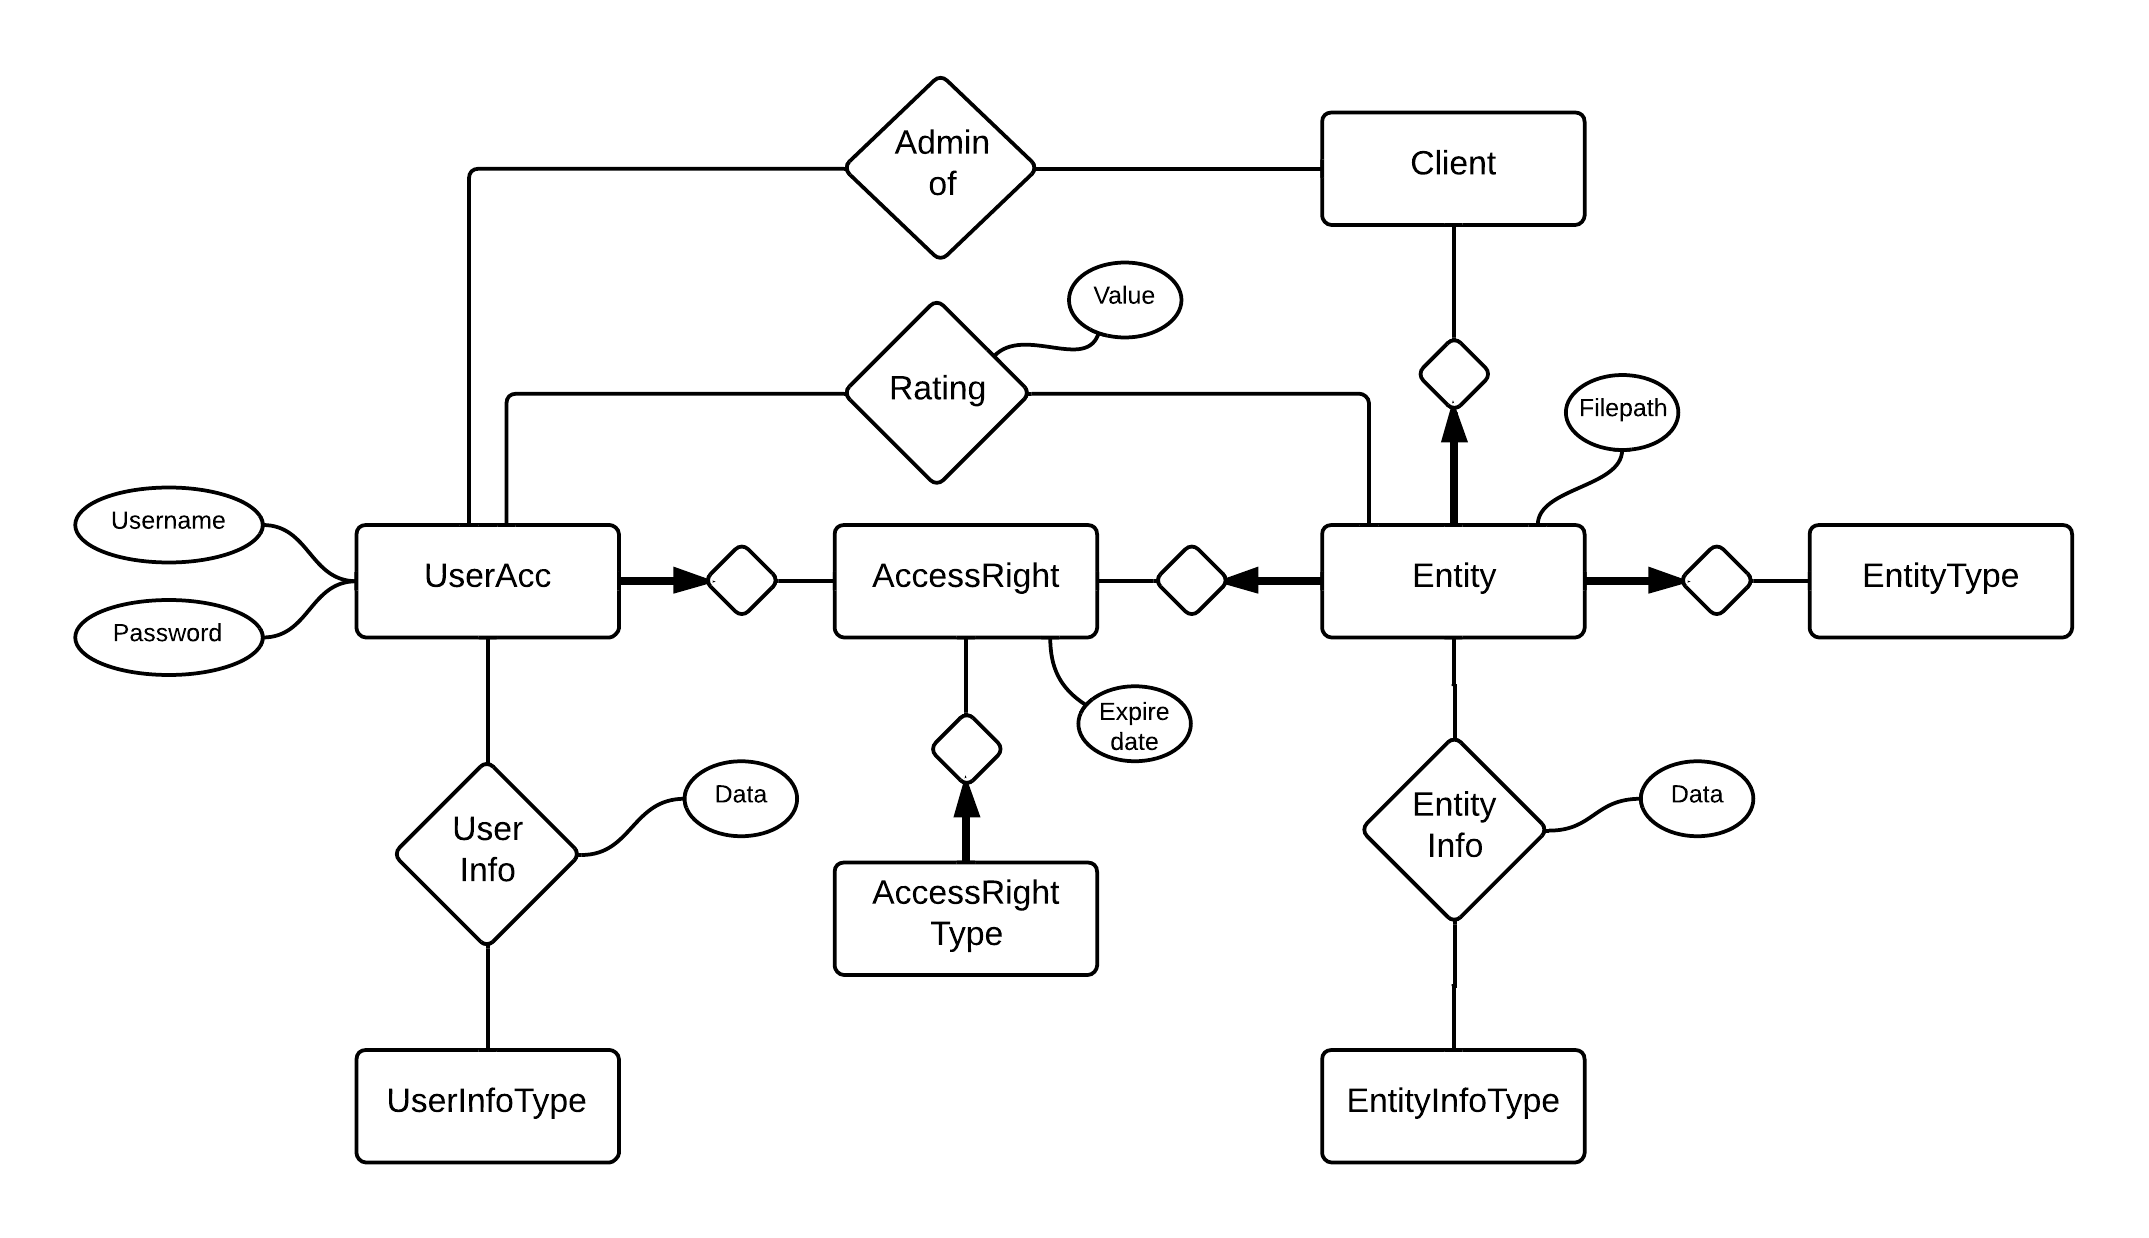
\includegraphics[width=\linewidth]{ER.png}
\caption{ER diagram of the data model}
\label{fig:use case diagram}
\end{figure}

In order to make the data model flexible and extensible it was decided to only make the \textit{User} and \textit{Media item} carry required information while all other information, like title, artist, director, email etc., is made relational. This means that the \textit{Media item} is stored in three tables: Entity, EntityInfo and EntityInfotype (The SQL definition of \textit{Media Item} is shown fig \ref{datamodel}).

This facilitates the need clients might have concerning what information is stored in a \textit{User} or \textit{Media item} entity, as well as making it easier to add more information types iteratively.\\

\begin{figure}[H]
\begin{lstlisting}
CREATE TABLE EntityInfoType(
	Id Int IDENTITY Primary Key,
	Name varchar(256) NOT NULL,
);

CREATE TABLE Entity(
	Id Int IDENTITY Primary Key,
	FilePath varchar(256) NOT NULL,
	ClientId Int NOT NULL REFERENCES Client(Id) ON DELETE CASCADE,
	TypeId Int REFERENCES EntityType(Id)
);

CREATE TABLE EntityInfo(
	Data varchar(max),
	EntityId Int NOT NULL REFERENCES Entity(Id) ON DELETE CASCADE,
	EntityInfoTypeId Int NOT NULL REFERENCES EntityInfoType(Id) ON DELETE CASCADE,
	Id INT IDENTITY Primary Key
);
\end{lstlisting}
\caption{Snippet of Entity (\textit{Media item}) SQL definition}
\label{datamodel}
\end{figure}

Another design decision was to have an AccessRight relation between \textit{User}s and \textit{Media item}s. This choice was made to facilitate different access rights to a \textit{Media item} like Owner and Buyer.

The data model is in 3NF (Third normal form). It is in 3NF and not BCNF (Boyce-Codd normal form) because it has IDs on all entities. An ID for e.g. \textbf{EntityInfo} (See figure \ref{datamodel} for table definition) is not needed as it could have been a weak entity. It was given an ID because it made the implementation of a generic Data Access Layer easier.

The full data model SQL definition can be found in appendix

\end{document}